In this chapter, we will discuss the roadmap steps to carry out this work. First, we will reintroduce the work objectives. Finally, the work plan with the necessary steps to accomplish the proposed objectives.

\section{Objective}

As already discussed, we want to build models capable of making predictions regarding the evolution of discovered topics in a set of documents. We also want to find topics in real-time at each received document without having to redo the topic discovery process. Then, by the end of this work, we must have performed the tasks listed below.

\begin{itemize}
	\item Find a database long enough, over several years;
	\item Perform all necessary treatment steps to normalize the documents' texts;
	\item Find meaningful topics in a subset from the original database;
	\item Create a topic classifier to find out if a document addresses any topic of interest;
	\item Model topic evolution to evaluate the forecast accuracy.
\end{itemize}

\section{Research method}

With the objectives defined, we must have action plans to achieve them. Next, we will discuss in more detail the action plan for each of these previous punctuated steps.

We need to mention the figure notation used in the next sections. Whenever a box with the bottom right tip folded appears, it represents a machine learning process with all the applicable steps, such as cross-validation and hyperparameter tuning.

\subsection{Database}

The first necessary task is to find a database over several years. Some options are available, such as daily news from Wikipedia, newspaper articles, research and academic papers, patents, and even social media data like Twitter or Reddit. We must be careful to choose a database that covers several years in order to get a good temporal representation when modeling their topics.

\subsection{Pre-processing the data}

With the chosen database, we must define a data pre-processing pipeline to normalize the documents, putting all of then at the same pattern. For this, we can use the normalization techniques shown in Chapter \ref{chap:literature} like stemming, lemmatization, stop words removal, and all necessary textual manipulations to obtain the best text representation for the documents.

After processing the data, we need to index then over the time and, then, split the full treated data set in three subsets. They must be time ordered, as shown in Figure \ref{fig:database}, this means that for each document in $T_{i}$ its time index $t_{x}^{(i)}$ must be lower then any index $t_{x}^{(m)}$ in a document contained in $T_{m}$, and so on.

\begin{figure}[h!]
	\centering
	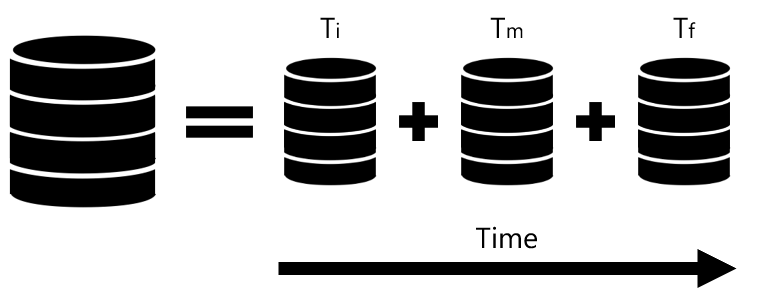
\includegraphics[width=0.6\linewidth]{01.Chapters/04.Materials/database}
	\caption{Database time split representation.}
	\label{fig:database}
\end{figure}

Before proceeding, let's name the subsets. The initial subset will be called \textit{Identifier} from now on, the middle and final ones will be respectively designated by \textit{Modeler} and \textit{Validation}. 

\subsection{Topic identification}

With the \textit{Identifier} set, techniques of document clustering will be applied to identify the discussed subjects in the documents, the Figure \ref{fig:topic-identification} illustrates the sequence of steps for this task. Similar to \citeonline{hurtado2016topic}, a refinement will be made so that only significant topics remain. 

\begin{figure}[h!]
	\centering
	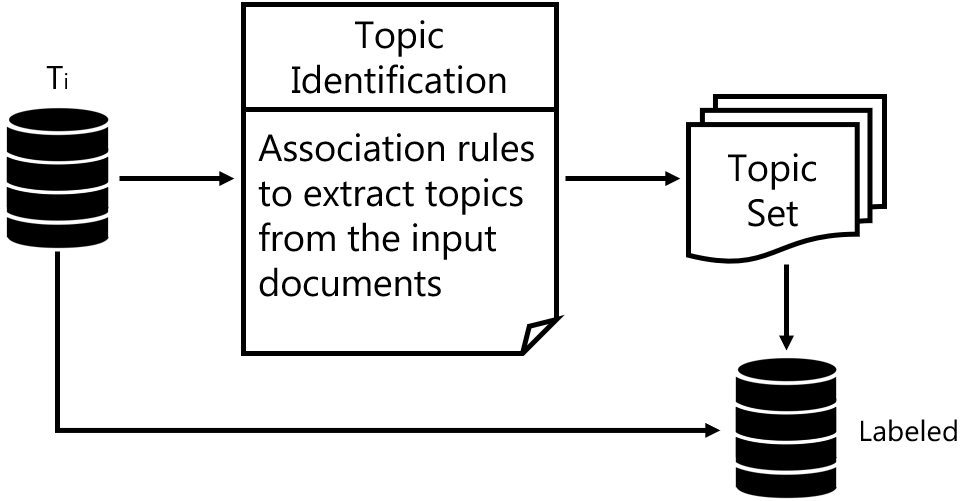
\includegraphics[width=0.8\linewidth]{01.Chapters/04.Materials/topic-identification}
	\caption{Topic identification process.}
	\label{fig:topic-identification}
\end{figure}

Next to the topic identification we will obtain a topic set, then each document contained in \textit{Identifier} can be labeled with at least one topic from the set, this new database will be called by labeled \textit{Identifier}.

\subsection{Document classification}

For each topic in our set of discovered topics, we must be able to identify which topics are covered by a new document. Thus, we will build a classifier to perform this verification.

Knowing that a document can talk about several topics, so we must have a multi-class classifier. We can see this as an individual binary classifier for each topic that tells us whether the document has it. Using the labeled \textit{Identifier} set it is possible to build this classifier. Figure \ref{fig:document-classification} illustrates it in detail.

\begin{figure}[h!]
	\centering
	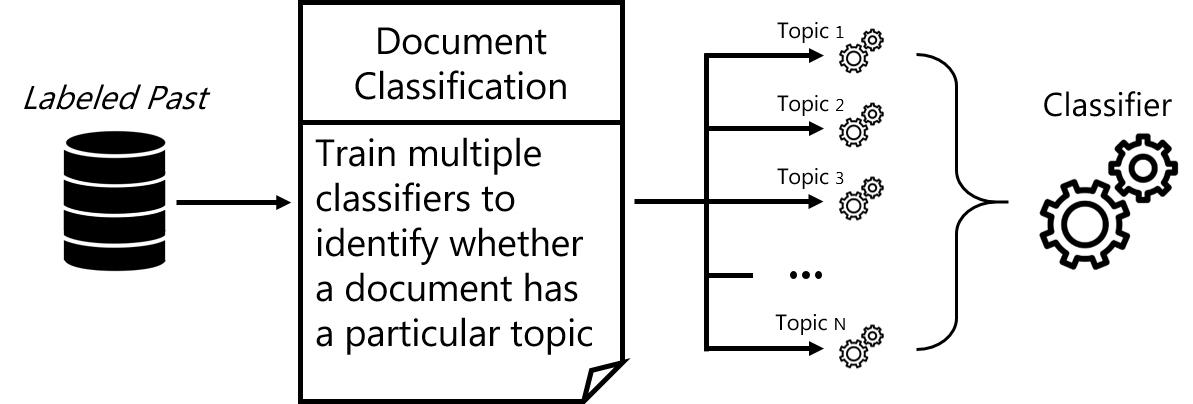
\includegraphics[width=0.9\linewidth]{01.Chapters/04.Materials/document-classification}
	\caption{Multi-class classifier from \textit{Labeled} set.}
	\label{fig:document-classification}
\end{figure}

\subsection{Forecast evaluation}

Finally, to evaluate the time series model is the last task to be accomplished. Following the flowchart shown in Figure \ref{fig:forecast}, first, we have to label the \textit{Modeler} and \textit{Validation} sets. Then, using labeled \textit{Identifier} and \textit{Modeler} we will build a topic incidence matrix over the time, to apply a forecaster process for those time series. With the labeled \textit{Validation} set we will perform an evaluation for our model and then make conclusions about it.

\begin{figure}[h!]
	\centering
	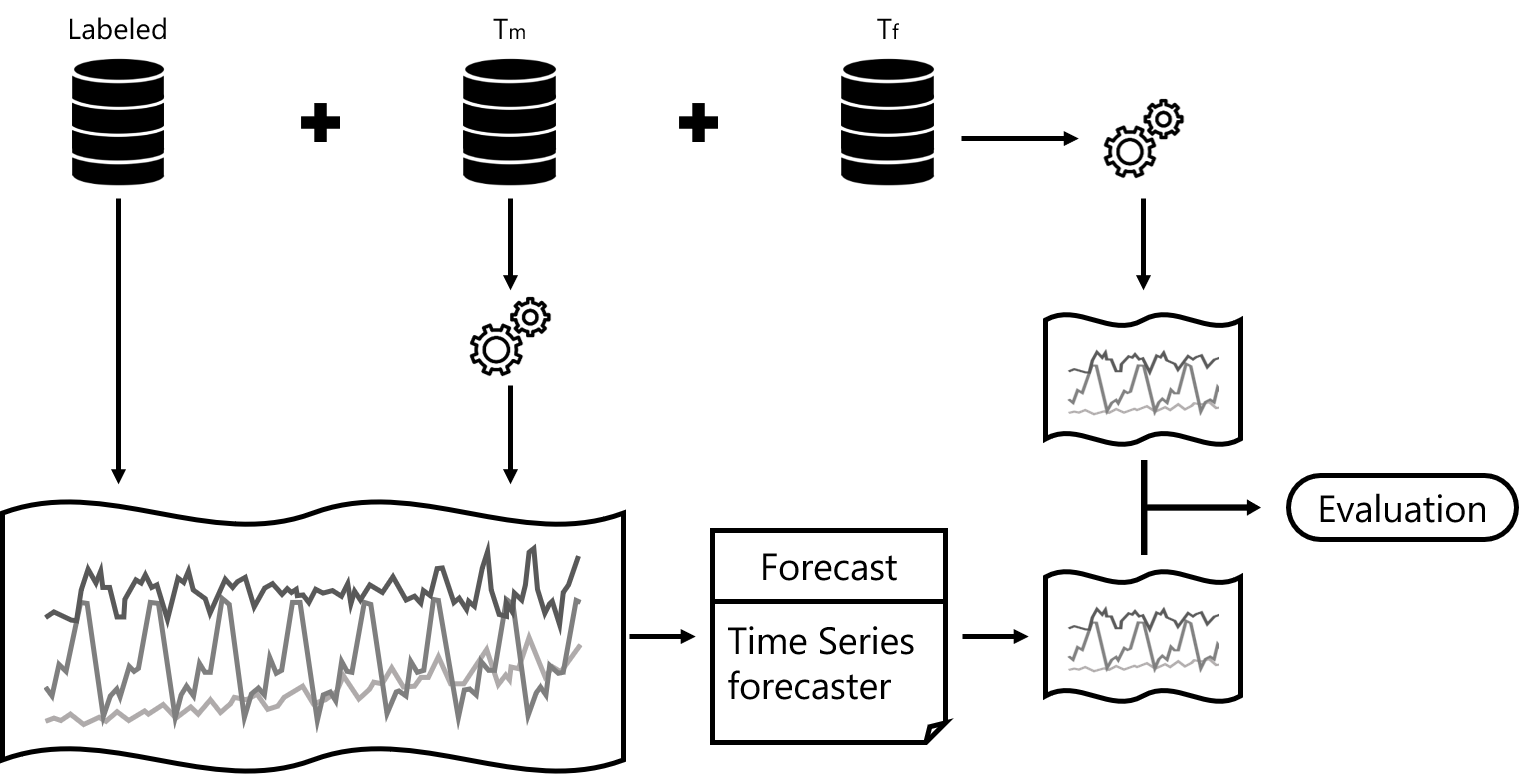
\includegraphics[width=\linewidth]{01.Chapters/04.Materials/forecast}
	\caption{Flowchart to evaluate the time series model.}
	\label{fig:forecast}
\end{figure}
